\chapter{心室的计算机辅助检测方法}
\label{chap:Detection}


计算机辅助检测(Computer-Aided Detections, CADs)是医学影像诊断过程中的一项重要任务,是进行相关结构功能测量的前提条件。其中,二维图像的目标组织结构自动检测是CADs技术的核心基础。在临床实践中,医生需整合不同模态、不同位置方向且以不同比例显示的图像信息,目前的研究主要关注如何使检测过程快速自动化。由于医学影像自身的特殊性,比如缺乏大量高质量标注数据;大多数医学目标组织结构存在非刚性形变;图像背景前景的区分不明显等,导致组织结构自动定位比较困难。现有大多数CADs系统在临床实际应用中表现不佳的原因是:检测结果的敏感性和特异性都较低,诊断效能低\citep{Cheng2016a}。


不同模态的医学图像中,如超声、计算机断层扫描(Computed Tomography, CT)和核磁共振(Magnetic Resonance Imaging, MRI)等,都存在目标身体器官自动定位的问题。以左心室(Left Ventricle, LV)检测为例,大多数LV定位方法主要依据位置,时间和形状的假设。基于位置的方法仅假设心室在图像的中心,该方法并不对不同病人心室位置的差异性以及图像的尺寸变化进行考虑,效果较差;基于时间的方法,假设左心室是图像中唯一的运动对象,然而这种方法敏感性高,除心室的运动伪影之外,还存在其它运动的器官,如Schollhuber\citep{Schollhuber2008}针对MRI短轴使用时空信息并消除运动伪影,由分层模式匹配算法定位包含LV的感兴趣区域,其通过使用互信息图像配准使运动伪影最小化,随后估计特征强度—时间曲线进行像素分类和边界的提取,得到最终分割结果;基于形状的方法将LV视为圆(短轴)、椭圆(长轴),然而该方法通常针对异常形状的LV容错性差,如Lu等\citep{Lu2009}使用大津阈值度量圆形程度,然后进行霍夫变换定位LV位置。也可搜索每个切片的质心,并用三维最小二乘拟合去除异常值,得到分割结果\citep{Petitjean2011}。


不依据具体的强先验假设,机器学习算法可通过区分前景目标对象和背景来解决目标结构自动检测的问题。如Kellman等\citep{Lu2011}提出了一种使用概率集成提升树来估计LV姿态和用空间间隔学习LV短轴边界的方法。Zhou等\citep{Zhou2005}在超声心动图中通过规一化集成提升回归学习非线性映射以定位LV,其团队后来提出针对多个器官的特异性置信最大化分类器,整合更高的自由度以改善回归定位任务的精度。Liu等\citep{She2007}通过利用基于子模块函数优化理论的多标记搜索策略来进行标记点的检测。Zheng等\citep{Zheng2014}在实现器官定位的同时,通过组合优化置信度来估计目标器官的位置、缩放及朝向等参数值。前述机器学习算法都基于弱先验知识,启发式设计相关特征,结合滑动窗口策略,选择分类器进行分类判断窗口中内容以估计相应位置。


近来通用物体检测领域取得巨大进展,主要得益于深度学习能利用大量标注数据,从原始像素出发,逐层分级学习中高层抽象语义特征\citep{Sharif2014}。区域卷积神经网络\citep{Girshick2014b}在大规模自然图像数据集(如ImageNet\citep{Russakovsky})上,识别性能远超传统方法\citep{Girshick2014b,Krizhevsky2012}。当前实践中由于深度学习需要大量的训练数据,所以仅在少数医学任务中取得有限的成功应用。深度学习方法用在定位检测问题时可分为两个阶段\citep{Girshick2015b}:候选框位置选取和窗口内容类别分类。如利用深度卷积网络进行显微镜图像中细胞检测\citep{Akram2016}、结合深度全卷积网络的MRI心室检测与分割\citep{Emad2015,Tran2016a}和超声图像解剖结构的检测\citep{Chen2016i}。这些方法大都关注特定目标结构的检测分割,而本文专门针对目前CADs普遍存在的检测定位问题,基于改进的生成候选框的快速区域深度卷积神经网络(Faster RCNN)\citep{Ren2015a}方法,提出一种医学目标结构检测框架:1)在区域生成网络的基础上引入空间变换损失使得候选框生成网络能捕捉目标的空间变换参数;2)采用在线困难样例挖掘策略,加快训练收敛过程,提高检测小目标的准确度;3)并基于目标先验知识,针对左心室提出利用检测二尖瓣环、心内膜垫和心尖位置,高效估计左心室姿态参数。4)为验证该算法的鲁棒性和有效性,分别针对两个具体CADs应用进行实验分析。

\section{区域卷积神经网络概览}
 
\subsection{物体检测形式化定义}
若用$r$来表示图像中的矩形窗口区域,令$R$表示由对象检测系统提供的所有候选窗口的集合,将有效定位标记定义为$R$的子集,使得标记位置内内容“不重叠”,令$Y$来表示所有有效标记位置的集合。并合并常用的非最大值抑制(Non-maximum suppression, NMS)过程,给定图像$x$和窗口评分函数$f$,物体检测算法流程可定义为:
\begin{table}[htbp]
 \caption{\label{tab:Algorithm1}物体检测算法流程 }
 \begin{center}
 \begin{tabular}{l}
  \toprule
  Input: 图像x,窗口得分函数f  \\
  \midrule
  1:  $D$:= 所有候选框 $r \in$ 使得$f(x, r) > 0$ \\
  2:  按 $f$ 排序$D$使得 $D1\geq D2 \geq D3 \geq ...Dn$ \\
  3:  令$y^∗:=\{ \}$   \\
  4:  for $i = 1$ to $n$ do \\
  5:     若 $D_{i}$ 和 $y^∗$中任意候选框不重叠 \\
  6:          $y^∗$ := $y^∗  \bigcup {D_{i}}$ \\
  7:  end for \\
  \midrule
  8:  Return:  $y^∗$,物体的目标位置. \\
  \bottomrule 
 \end{tabular}
  \end{center}
\end{table} 
 
形式化定义物体检测过程见公式\ref{eq:ch05_01},式中参数定义请参考算法\ref{tab:Algorithm1}。
\begin{equation} \label{eq:ch05_01}
      y^∗=\mathop{\arg\min}_{y\in Y}\sum _{r\in Y} f(x,r)
\end{equation}                               	 
通常公式\ref{eq:ch05_01}可通过贪心搜索的方法来完成,算法将联合最小化在算法\ref{tab:Algorithm1}中产生假阳例的数量和最大化检测窗口评分函数,即寻找具有最大得分但同时不重叠的滑动窗口位置集合。
\subsection{区域卷积神经网络的演进}

2014年Gisrshick等\citep{Girshick2014b}提出区域卷积神经网络(Region-based Convolutional Neural Network, RCNN),对每一候选框窗口都进行一次前向传播,这将导致冗余计算,时间复杂度高,为解决这一问题,He和Ren等提出SPP-net\citep{He2015spp}和Fast RCNN\citep{Girshick2015b}加以改进,不再把每一候选窗口均送入网络,而是仅对图像特征提取一次,把原图中候选区域投影到卷积特征图上,然后对投影后的区域特征图进行空间感兴趣区域池化(ROI Pooling)得到固定长度的特征向量。其中Fast RCNN中的感兴趣区域池化是SPP-Net中多尺度空间金字塔池化的特例,仅用单一尺度的金字塔池化操作。RCNN及其改进的Fast RCNN都依赖于人为设计的候选框生成方法,如选择性搜索等。为减少生成候选框的计算时间,Faster RCNN提出区域生成网络(Region Proposal Networks,RPN),区域生成网络和检测网络共享提取特征的卷积层,仅提取几百个或者更少的高质量预选窗口,且召回率较高(导致更少的假阳例)。但现有的通用物体检测算法均是假设候选框为矩形,不能解决旋转朝向问题。

 
\section{候选区域生成网络及其改进}
 
本章将分别从候选区域生成网络模型的结构、仿射变换候选框区域的生成、空间变换损失函数的设计、模型训练方法等方面介绍本文所提出框架,并结合Faster RCNN模型提出端到端的目标检测方法。

\subsection{候选区域生成网络模型结构}

候选区域生成网络将一图像(任意大小)作为输入,输出目标候选框的集合和每个候选框内有无目标的概率估计,如图\ref{fig:ch05_01}右图所示,RPN在卷积层后接两个全卷积层完成候选区域生成功能,以实现增加滑动窗口操作。该模型使用全卷积网络[20]处理任意大小的图片输入,为了和目标检测网络\citep{Girshick2015b}共享计算,在特征提取的过程中同时计算目标检测所需的感兴趣区域的初始估计,在最后一个共享卷积层输出的特征映射图上滑动小网络,卷积特征映射图上n×n大小空间窗口作为该网络全连接的输入,本文n取3。每个滑动窗口映射到一个低维向量上(如图\ref{fig:ch05_01}左上中256-d),该向量输出给两个全连接层——候选框位置定位回归层和候选框类别分类层。原文中采用类别无关分类损失,即仅区分该候选框内是否包含物体(前/背景),本文将其扩展为类别相关的分类损失。
\begin{figure}[!htbp]
\centering
%trim option's parameter order: left bottom right top
%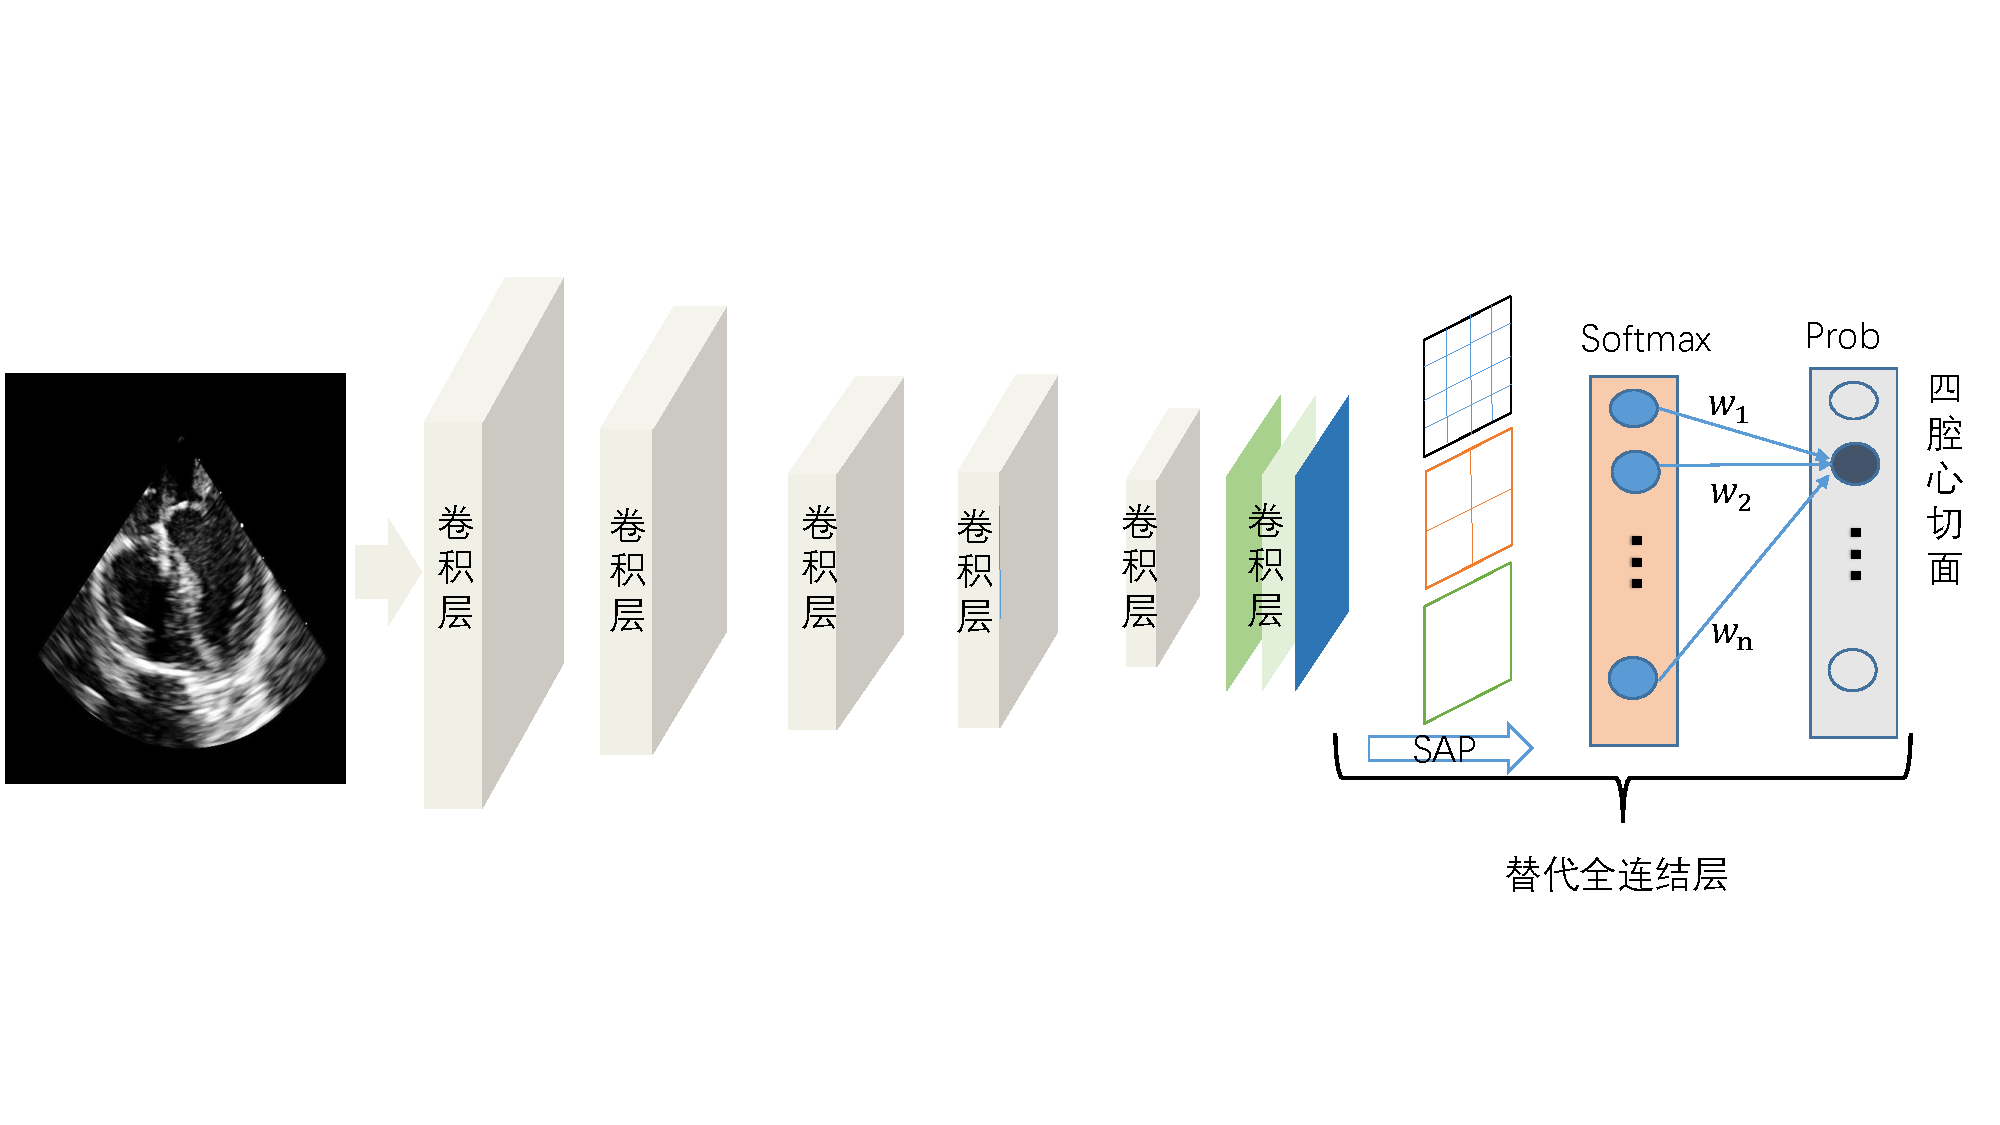
\includegraphics[trim = 30mm 0mm 30mm 0mm, clip, width=0.45\textwidth]{ch03_02}
\includegraphics[width=0.85\textwidth]{ch05_01}
\caption{左上:引入空间不变性的anchor机制\   左下:空间变换网络  右:Faster R-CNN带仿射变换的检测模型框架}
\label{fig:ch05_01}
\end{figure}

为引入空间尺度不变性,采用多尺度和多纵横比的“参考”框(anchor)(图\ref{fig:ch05_01}左上所示)。该机制可看作是金字塔型参考框的回归,避免了枚举多尺度、多纵横比的图像或卷积核。在每一个滑动窗口的位置,同时预测$k$个参考区域,回归层有$4k$个输出,即$k$个box的坐标编码,多元逻辑回归分类层输出$(c+1)×k$个(物体类别数$c$加背景类的)概率估计。候选框由相应的$k$个anchor的参数化表示,每个anchor以当前滑动窗口中心为中心,并对应一种尺度和长宽比,我们使用3种尺度和3种长宽比,在每一个滑动位置就有$k=9$个anchor。对于大小为w×h的卷积特征映射,总共有$w×h×k$个anchor。

\begin{figure}[!htbp]
\centering
%trim option's parameter order: left bottom right top
%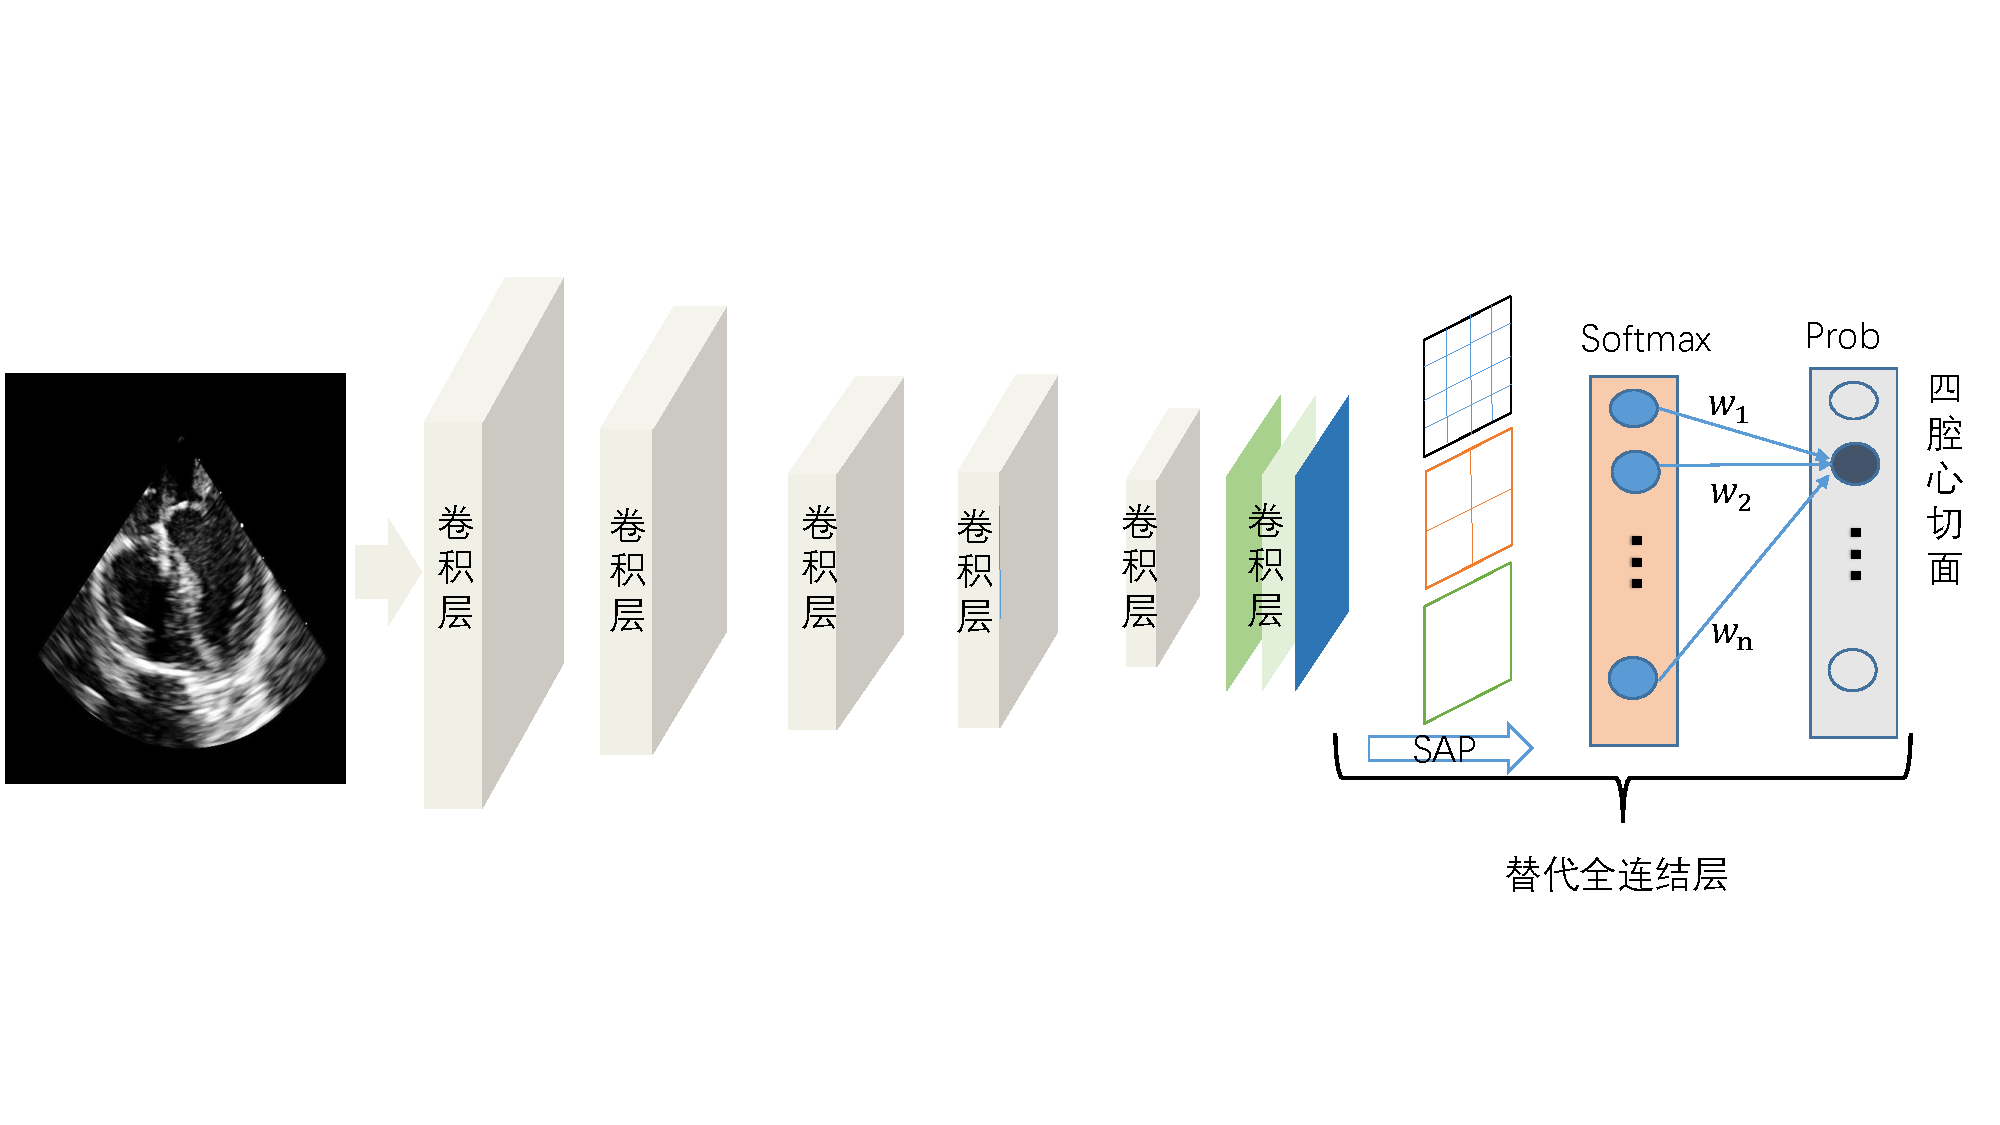
\includegraphics[trim = 30mm 0mm 30mm 0mm, clip, width=0.45\textwidth]{ch03_02}
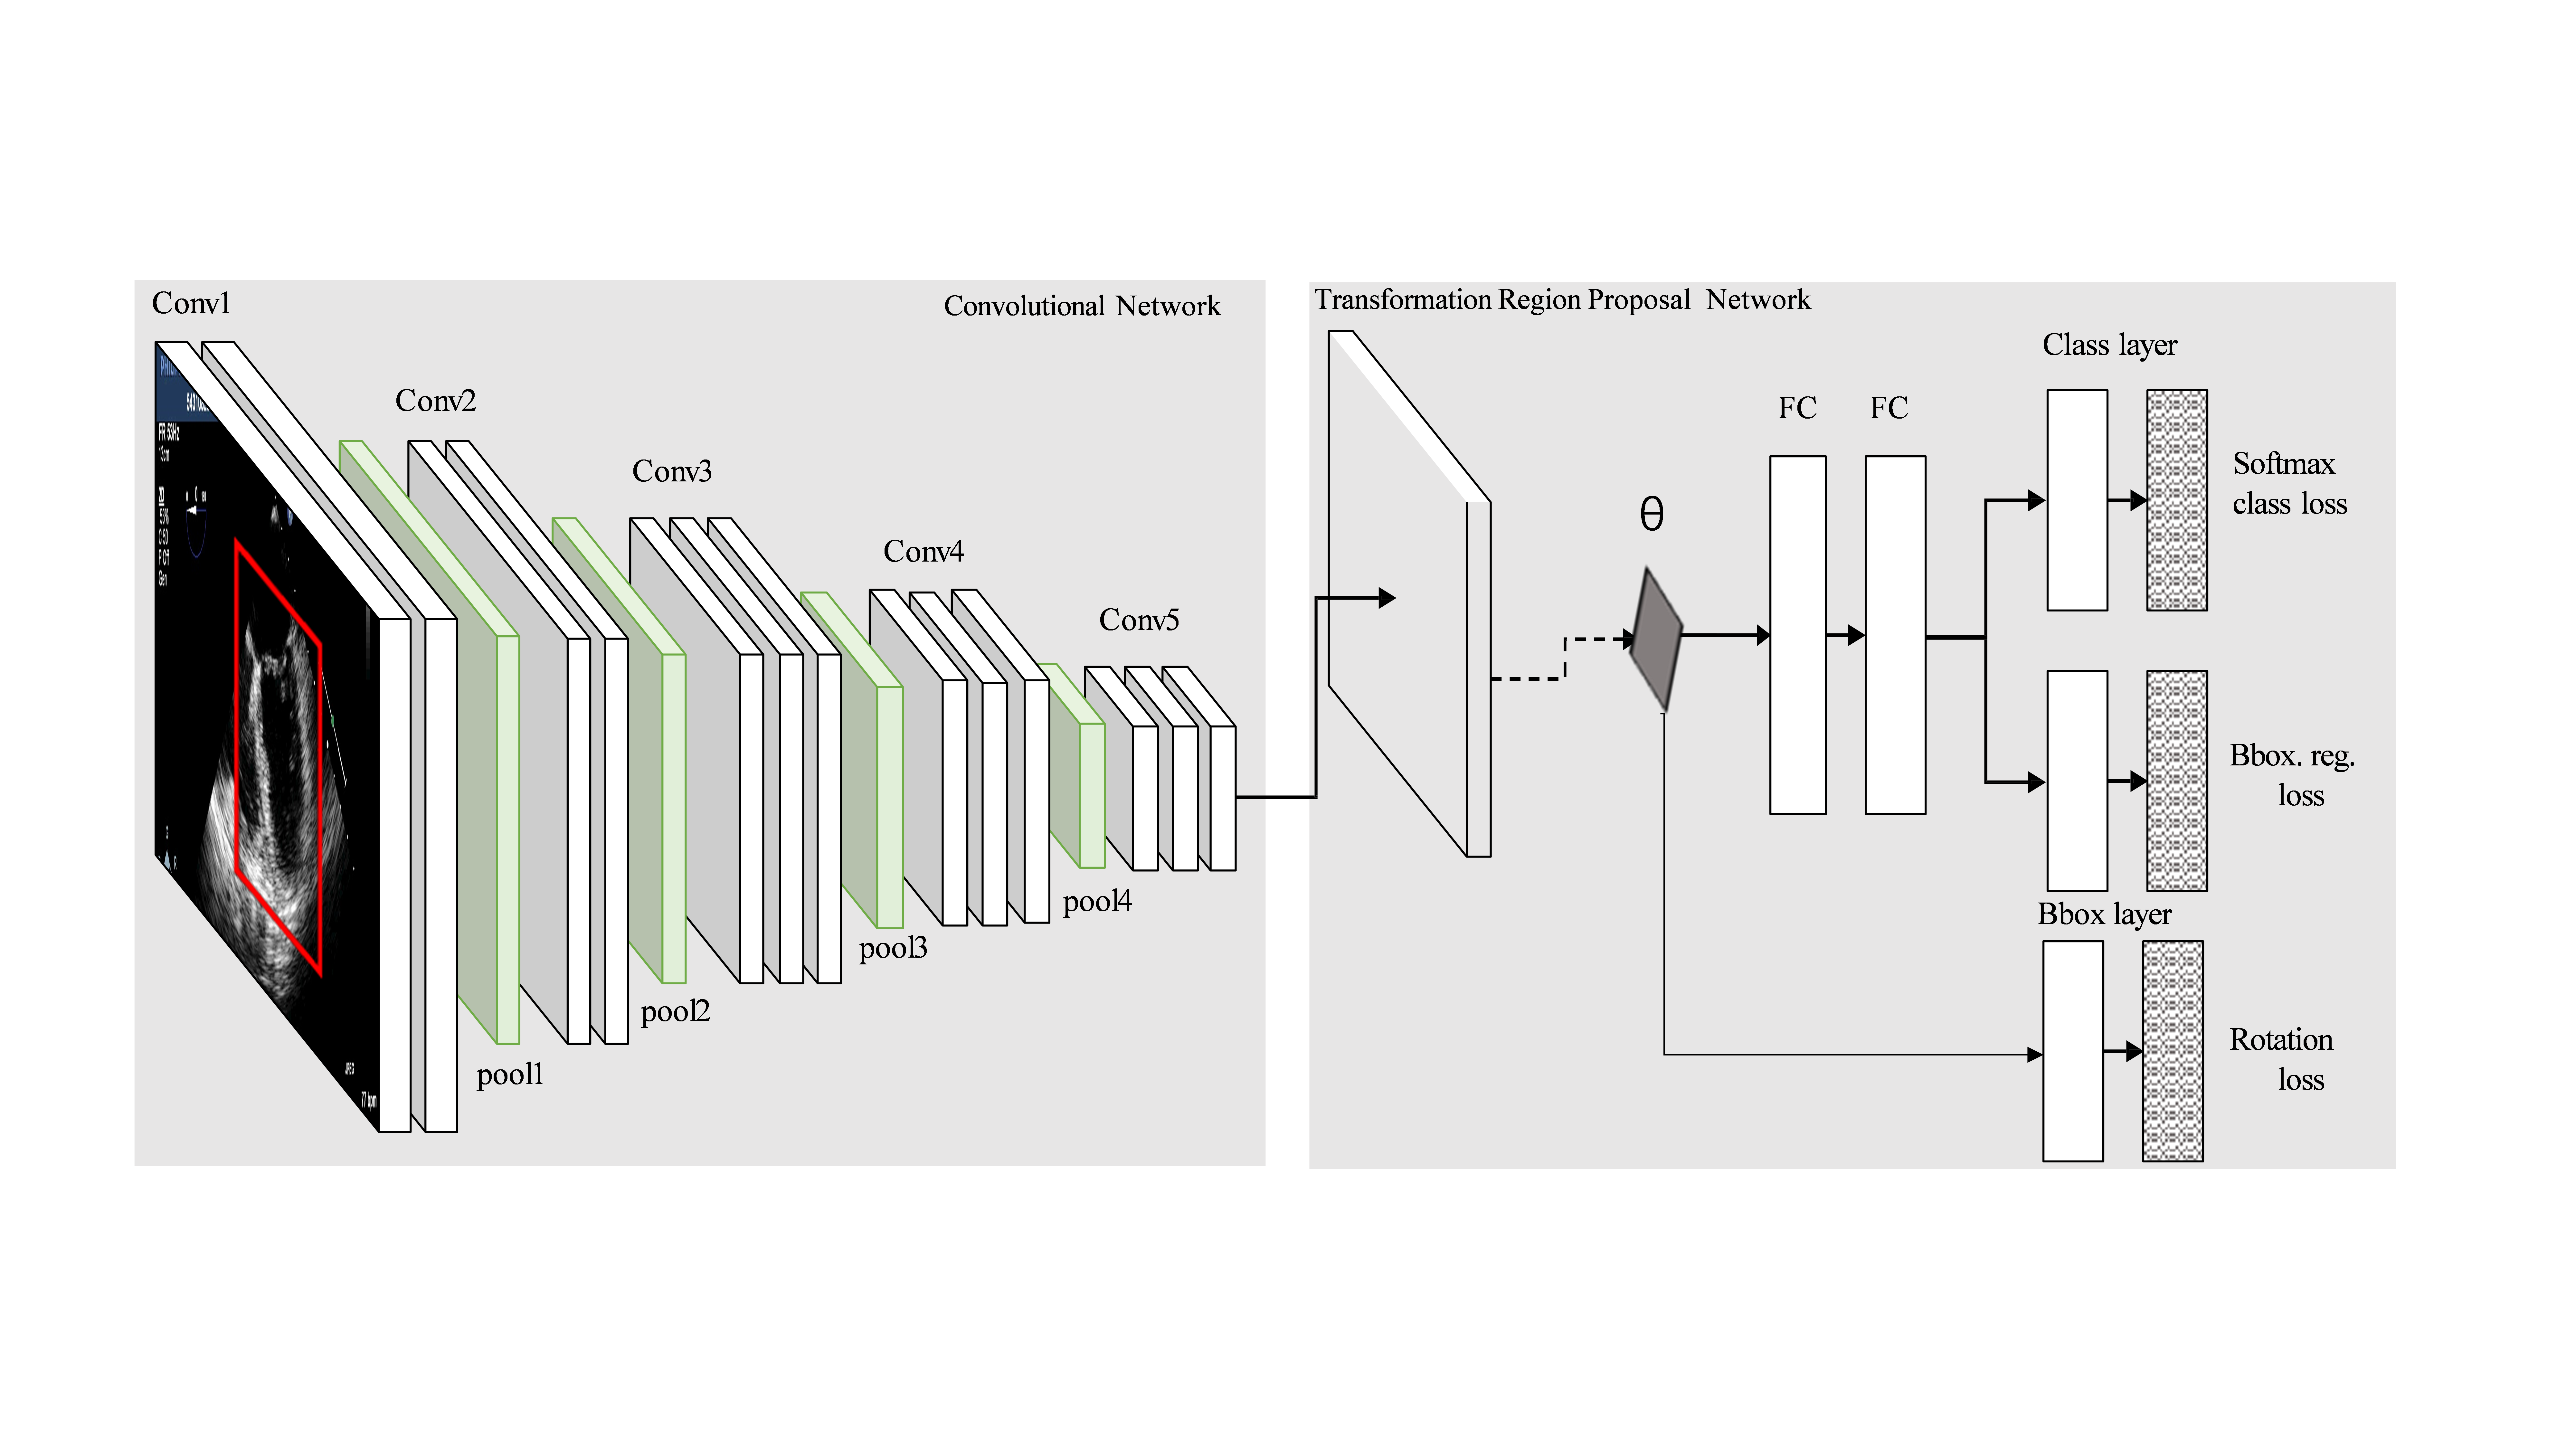
\includegraphics[trim = 30mm 0mm  30mm 0mm,width=0.95\textwidth]{ch05_02}
\caption{考虑物体朝向的区域生成网络模型结构示意图,图中conv表示卷积层,pool表示池化层,FC表示全连接层,softmax class loss表示多任务损失中的分类损失,Bbox.reg loss 表示候选框回归定位损失,Rotation loss表示文中的针对变换参数θ的Von Mise损失。}
\label{fig:ch05_02}
\end{figure} 

\subsection{仿射变换候选框}
 
为检测物体的姿态,结合空间变换网络\citep{Jaderberg2015}(见图\ref{fig:ch05_01}左下),提出带仿射变换的候选框生成算法。之前的候选框生成方法仅考虑固定尺度和宽高比的矩形框,并未考虑物体的旋转朝向,二维空间仿射变换可表示为:
\begin{equation} \label{eq:ch05_02}
\begin{pmatrix}
x_{i}^{s}\\ 
y_{i}^{s}
\end{pmatrix} =\tau _{\theta}\begin{pmatrix}
x_{i}^{t}\\ 
y_{i}^{t}\\
1
\end{pmatrix}=\begin{bmatrix}
\theta_{11} &\theta_{12}  &\theta_{13} \\ 
 \theta_{11}&\theta_{22}  & \theta_{23}
\end{bmatrix}\begin{pmatrix}
x_{i}^{t}\\ 
y_{i}^{t}\\
1
\end{pmatrix}
\end{equation}                    
式中$(x_{i}^{s},y_{i}^{s})^T $为输入特征图中目标坐标系下的网格点,$\tau _{\theta}$ 为变换矩阵, $(x_{i}^{t},y_{i}^{t})^T $为输出特征图中目标坐标系下的采样网格点。其中由于图像的坐标不是中心坐标系,宽高坐标需归一化表示,如$-1\leq x_{i}^{s},y_{i}^{s}\geq 1$ ,且采用图形学中齐次坐标表示。公式\ref{eq:ch05_02}能用六个参数定义对输入特征图的裁剪、平移、旋转和缩放等变换。该公式进步简化为只考虑旋转变换:
\begin{equation} \label{eq:ch05_03}
\begin{pmatrix}
x_{i}^{s}\\ 
y_{i}^{s}
\end{pmatrix} =\tau _{\theta}\begin{pmatrix}
x_{i}^{t}\\ 
y_{i}^{t}\\
1
\end{pmatrix}=\begin{bmatrix}
\cos\alpha &-\sin\alpha  &0 \\ 
 \sin\alpha&\cos\alpha  & 0
\end{bmatrix}\begin{pmatrix}
x_{i}^{t}\\ 
y_{i}^{t}\\
1
\end{pmatrix}
\end{equation}  
其中 $\alpha$表示绕图像中心顺时针旋转角度,通常变换后的像素并不是在相应网格的整数值,常用双线性插值进行近似,变换后的候选框送入感兴趣区域池化层,后接多任务损失函数。实质是把空间变换层嵌入到RPN网络中,并且引入有监督的损失以指导空间变换。
\subsection{朝向回归损失函数}

旋转朝向的周期性会导致两个问题:(1)要优化的损失函数不能区分对于周期性损失,简单地将模运算符应用于网络的输出会导致不可靠的损失,不能再被鲁棒地优化。(2)由大多数参数模型中执行的矩阵向量积产生的回归输出是固定的线性运算。为此提出旋转朝向回归损失$L_{VM}(o,o^{*})$ ,第一个问题可以通过采用Von Mise 分布\citep{Beyer2015}来解决损失函数不连续性,其近似服从于单位圆上的正态分布:
\begin{equation} \label{eq:ch05_04}
      p_{VM}(\varphi \mid \mu,k)=\frac{e^{k \cos(\varphi-\mu)}}{2\pi I_{0}(k)}
\end{equation} 	                            	  					             
其中$p$指相应的概率密度函数,$\varphi$ 指角度,$\mu $ 是分布的平均角度,$k$ 与近似高斯方差成反比,而$I_{0}(k)$  是阶数为0的修正贝塞尔函数,利用余弦函数来避免不连续性,可以得出以下损失函数:
 \begin{equation} \label{eq:ch05_05}
      C_{VM}(\theta \mid t,k)= 1- e^{k (\cos(\theta-t)-1)}
\end{equation}         			                    
式中$\theta$ 为预测旋转角度大小,$t$为真实旋转角度大小,称$t$为目标值,$k$为控制损失函数尾部的简单超参数。由角度$varphi$ 正余弦组成的二维向量$y=(\cos\varphi,\sin\varphi)$ 替代表示,利用自然语言处理文献中广泛使用的余弦代价函数[31]来解决使用线性操作来预测周期值的问题:
\begin{equation} \label{eq:ch05_06}
     C_{\cos}(y \mid t)=1- \frac{y\times t}{\parallel y\parallel \parallel t\parallel}  
\end{equation}      					               
在神经网络框架中的实现是相对简单的,因为所需要的是全连接层和归一化层,前向传播公式:
\begin{equation} \label{eq:ch05_07}
      f_{BT}(x \mid W,b)=\frac{Wx+b}{\parallel Wx+b \parallel }
\end{equation}  
                     			                    	 
式中 $W\in R^{n\times 2}$ 和 $b\in R^{2}$ 是来自全连接层的可学习参数,然后反向传播归一化损失的导数为
\begin{equation} \label{eq:ch05_08}
      \partial _{x_{i}} \frac{x}{\parallel x\parallel}=\partial _{x_{i}}\frac{x }{\sqrt{\sum_{j}x_j^2}} =\frac{\sum_{j \neq 
 i}x_j^2 }{(\sum_{j}x_j^2)^{\frac{3}{2}}}  =\frac{\sum_{j \neq i}x_j^2 }{\parallel x\parallel^3} 
\end{equation} 	                 			    
式中归一化确保输出值被联合学习,通过比较$CVM$和$Ccos$,最终朝向回归损失函数为
\begin{equation} \label{eq:ch05_09}
      L_{VM}(y\mid t) = 1- e^{k (y\times t-1)}
\end{equation} 	                           								
与式\ref{eq:ch05_06}相似,主要区别在于存在e,它将目标值附近的错误“下推”,实际上是较小地惩罚小错误。

\subsection{带朝向的多任务损失函数}

多任务损失分别存在于RPN及检测网络中,图2中显示的是检测网络结构示意图。每一个候选框均送感兴趣池化层,后接两层的全连接层和多元逻辑回归分类损失(图\ref{fig:ch05_02}中Softmax loss),候选区域回归定位损失(图\ref{fig:ch05_02}中Box.reg loss)和旋转朝向回归损失(图\ref{fig:ch05_02}中Rotation loss):
\begin{equation} \label{eq:ch05_10}
      L(p,p^*,t,t^*,o,o^*)=L_{cls}(p,p^*)+\lambda[p^*> 0]L_{box}(t,t^*)+\mu [p^*> 0]L_{VM}(o,o^*)
\end{equation} 

式中,分别代表预测类别分类概率,候选框偏移量和感兴趣区域内物体的朝向大小; 表示标记类别为背景, 表示框内是否有目标的指示函数, 分别表示物体的候选框标记和真实朝向。 为两个损失的相应平衡权重大小,详细形式如下:
 \begin{equation} \label{eq:ch05_11}
      L_{(cls)}(p,p^*)=-\sum_{c}\log p_{c}^*
\end{equation} 

 \begin{equation} \label{eq:ch05_12}
      L_{box}(t,t^*)=-\sum_{i \in {(x,y,w.h)}}smooth_{L1}(t^*-t)
\end{equation} 

\begin{equation} \label{eq:ch05_13}
smooth_{L1}(x)= \left\{
     \begin{matrix}
0.5x^2 & if \mid x\mid<1 \\
 \mid x\mid-0.5 & else \\
\end{matrix}\right.
\end{equation} 

 $L_{cls}(p,p^*)$和$L_{box}(t,t^*)$ 是公式\ref{eq:ch05_04}中的分类损失和相应的平滑L1损失,$c$代表类别数。
\subsection{困难样例挖掘}

由于医学数据样本标注困难,数量相对较少,一般假设与目标位置矩形框有重叠的候选框是有较大概率是难以区分的,结果也可能是次优的,因为在其他位置可能存在更难区分的样本,导致模型收敛变慢,误警率高。在每次迭代训练过程中采用在线困难样例挖掘方法(Online Hard Example Mining,OHEM)\citep{Shrivastava2016a},对所有候选框的损失进行排序,由于相似候选框重叠区域的损失很接近,可采用非极大值抑制策略限制候选框的数目,选择前$k$个最大损失作为困难样例,反向传播其相应的梯度,其他候选框的梯度不进行回传,即不更新模型权重。 

\section{实验结果分析和讨论}
 
为验证提出的自动检测算法的有效性和正确性,本节将分别采用一个公开可用的MRI数据集,和我们收集的来源于四川大学华西医院麻醉科的经食道超声心动图数据集(不包含患者信息)上进行实验。相关实验代码请参考\footnote{https://github.com/taopanpan/echodetection}。

\subsection{检测MRI左心室短轴}

纽约大学提供的公用数据集\citep{Andreopoulos2008}包含33名患者的心脏MRI体数据,以及LV心内膜和心外膜的手动分割结果。该数据集中的大多数切片包含心脏疾的病例切片。该数据集使用 GE Genesis Signa MRI扫描仪,采取FIESTA方案扫描获得。每个患者的20个序列帧包含8-15个短轴切片,大小为256x256,厚度为6-13 mm,像素分辨率为0.93-1.64 mm。为了检验所提出方法定位性能,取14个体数据形成1176个切片作为训练集,其余作为测试集。本实验中不使用旋转朝向损失,评价指标采用文献\citepns{Emad2015}中定量评估计算左心室短轴(SAX)定位的准确度,敏感性和特异性。

\begin{table}[!htbp]
    \centering
    \footnotesize% fontsize
    \setlength{\tabcolsep}{4pt}% column separation
    \renewcommand{\arraystretch}{1.2}%row space 
    \begin{tabular}{lccc}
        \cline{1-4}% partial hline from column i to column j
           \qquad Method  & Accuracy & Sensitivity &Specificity \\
        \hline
        Baseline\citep{•} & $95.06\%$ & $73.91\%$ & $97.56\%$\\
        \hline
        VGG16 & $96.35\%$ & $74.68\%$& $99.26\%$ \\
        \hline
        ResNet101 & $98.66\%$ & $76.81\%$& $99.16\%$ \\
        \hline
        VGG16\_OHEM & $96.56\%$ & $79.42\%$& $99.07\%$ \\
        \hline
        ResNet101\_OHEM & $\textbf{99.49\%}$ & $\textbf{83.12\%}$ & $\textbf{99.40\%}$\\
        \hline\hline
    \end{tabular}
    \caption{不同模型检测精度的比较}
    \label{tab:ch05_02}
\end{table}

为评价不同深度模型对检测效果的影响,实验的检测模型选取VGG16\citep{Simonyan2014a}和ResNet101\citep{he15},训练方法采取端到端的近似联合优化,OHEM表明训练过程中采用困难样例挖掘方法,即在训练中只选择损失占前70\%的样本进行反向传播。训练参数及实现跟文献\citepns{Ren2015a}中一致,迭代次数为1000,以文献\citepns{Ren2015a}方法作为基准(表\ref{tab:ch05_02}中Baseline),评价指标采用通用的定位精度、敏感性和特异性,结果见表\ref{tab:ch05_02}所示,在测试集上最优检测准确度99.49\%,敏感性83.12\%,特异性为99.40\%,与基准检测模型相比精度提高了超过3\%,同时提高了约1.5\%的特异性。
另一方面,敏感性是最容易提高的参数,平均超过8\%,模型不能正确定位为大尺寸的心脏,导致较小LV切片的高FP,降低了整体系统性能。而困难样例挖掘的方法没有显著提高特异性,因为TN和FP都降低。考虑到心脏异常的高变异性导致心脏形状的大变异性,所提出的算法均能成功定位LV短轴,当检测出心室短轴时,可大致确定心室中心点(如图\ref{fig:ch05_04}(a)所示),利用二腔心(2CH)和四腔心切面(4CH)均垂直于短轴切面的先验,找到与SAX的2CH和4CH交集在SAX平面上投影,然后得到投影线在2D图像上相交的位置,即为左心室的3D位置(如图\ref{fig:ch05_04}(b)所示)。
\subsection{检测左心室及其朝向}

MRI左心室短轴的检测由于组织结构相对简单,且噪声少。为验证提出算法的通用性,针对超声图像左心室长轴切面检测心室、二尖瓣环、心内膜垫和心尖位置,并估计左心室朝向。主要包含单扇形和多普勒成像的双扇形两种由专业医师标注食管中段四腔心(ME4C) 的标准切面视频构成,视频中至少包含2-3个心动周期,依据医师建议从视频中截取5帧,并经医师检验手工筛选后得到900张ME4C切面,对切面内左心室(LV),二尖瓣环、心内膜垫和心尖位置进行人工标注作为“金标准”。其中随机选取100张作为测试集,其余作为训练集。
训练时采用提出的联合多任务损失,以VGG16网络作为检测的预训练的模型为例,在RPN中添加空间变换网络实现了各个候选框的空间变换,并施加旋转朝向损失。VGG16网络特征提取器包括13个卷积层,并输出512个conv5特征图,空间变换网络包括具有两个同样卷积池化层组成的定位网络,其由20个卷积核大小为5、步长为1和核大小为2的池化层构成,两层全连接层回归得出6个仿射变换参数,其中,全连接层的激活函数需选择为双曲正切函数,权重高斯初始化,而变换参数初始化为$[1 0 0 0 1 0]^T$。其它跟Faster RCNN中设置一致,其中$\lambda$、$\mu$, 分别取0.1和0.001;训练方法采取端到端的近似联合优化,迭代轮数为50000。评价指标采用平均检测精度(mean average precision,mAP),是多个类别平均检测精度的平均值。表二显示使用提出方法分别在VGG16模型和ResNet101模型上,结合困难样例挖掘训练方法得出的测试结果,其中OHEM表示相应模型结合在线困难样例挖掘方法的检测结果,STN表示结合提出带朝向损失的空间变换网络的检测结果,在测试集上,针对左心室的AP最优可达99.12\%,结果表明提出算法在不同基础模型上均可提高检测精度。

\begin{table}[!htbp]
    \centering
    \footnotesize% fontsize
    \setlength{\tabcolsep}{4pt}% column separation
    \renewcommand{\arraystretch}{1.2}%row space 
    \begin{tabular}{lccccc}
        \cline{1-6}% partial hline from column i to column j
           \qquad Method  & MAP & lv &apx &left &right\\
         
        \hline
        VGG16\_OHEM & $80.11\%$ & $90.12\%$& $65.46\%$ & $81.27\%$& $83.53\%$\\        
        \hline
        VGG16\_OHEM\_STN & $82.05\%$ & $90.92\%$& $66.57\%$& $86.16\%$& $84.46\%$ \\
        \hline
        ResNet101\_OHEM & $83.06\%$ & $95.72\%$& $66.39\%$& $85.25\%$& $84.83\%$ \\
        \hline
        ResNet101\_OHEM\_STN & $\textbf{85.59\%}$ & $\textbf{99.12\%}$ & $\textbf{67.89\%}$ & $\textbf{87.66\%}$ & $\textbf{87.48\%}$\\
        \hline\hline
    \end{tabular}
    \caption{不同模型检测精度,LV表示左心室,Apx代表心尖,left代表二尖瓣环,right代表心内膜垫}
    \label{tab:ch05_03}
\end{table}


为验证提出算法在检测左心室位置的同时可以回归学习左心室的姿态参数、预测左心室的朝向变换,超参数k跟文献\citepns{Beyer2015}一致,交叠比大于0.5时估计姿态参数,人为标定心室朝向存在较大偏差,但可以根据二尖瓣环、心内膜垫和心尖位置估算出心室朝向角度作为对照。由于ME4C切面中心室的大概朝向的分布范围在$[-45^{\circ},45^{\circ}]$之间,通过手工构建训练集,训练样本旋转以$15^{\circ}$为间隔的指定角度。通过分析相关估算结果和预测结果,可以发现二者具有很大的一致性。左心室检测结果和旋转朝向结果见表\ref{tab:ch05_03},检测结果如图\ref{fig:ch05_04}(c,d)所示,更多实验结果请参考给定开源地址。
\begin{table}[!htbp]
    \centering
    \footnotesize% fontsize
    \setlength{\tabcolsep}{4pt}% column separation
    \renewcommand{\arraystretch}{1.2}%row space 
    \begin{tabular}{lccccccc}
        \cline{1-8}% partial hline from column i to column j
           \qquad Method  & $-45^{\circ}$ & $-30^{\circ}$ & $-15^{\circ}$ & $+15^{\circ}$ & $+30^{\circ}$&$ +45^{\circ}$& Avg\\
         
        \hline
        Compute & $66.65\%$ & $78.02\%$& $87.39\%$& $85.53\%$& $75.83\%$ &$62.31\%$ &$75.94\%$  \\
        \hline
        Pred & $\textbf{73.09\%}$ & $\textbf{81.72\%}$ & $\textbf{81.75\%}$ & $\textbf{89.56\%}$ & $\textbf{80.48\%}$& $\textbf{70.31\%}$& $\textbf{80.76\%}$\\
        \hline\hline
    \end{tabular}
    \caption{不同旋转角度分类检测性能比较,Compute表示根据额外标记计算得到的结果,Pred表示模型预测结果}
    \label{tab:ch05_04}
\end{table}

为了更详细地评估模型性能,使用检测分析工具\citep{Hoiem2012}分析了心尖位置的检测结果,如图\ref{fig:ch05_03}显示模型可以准确(白色区域)检测到心尖位置,召回率在84-87\%左右,并且比“弱”标准(小于0.1交叠比)高得多。针对心尖位置的定位精确度较低,这是因为医师在标定心尖位置时有很大的随意性,且目标尺寸较小,与类似对象类别有更多的混淆。
\begin{figure}[!htbp]
\centering
%trim option's parameter order: left bottom right top
%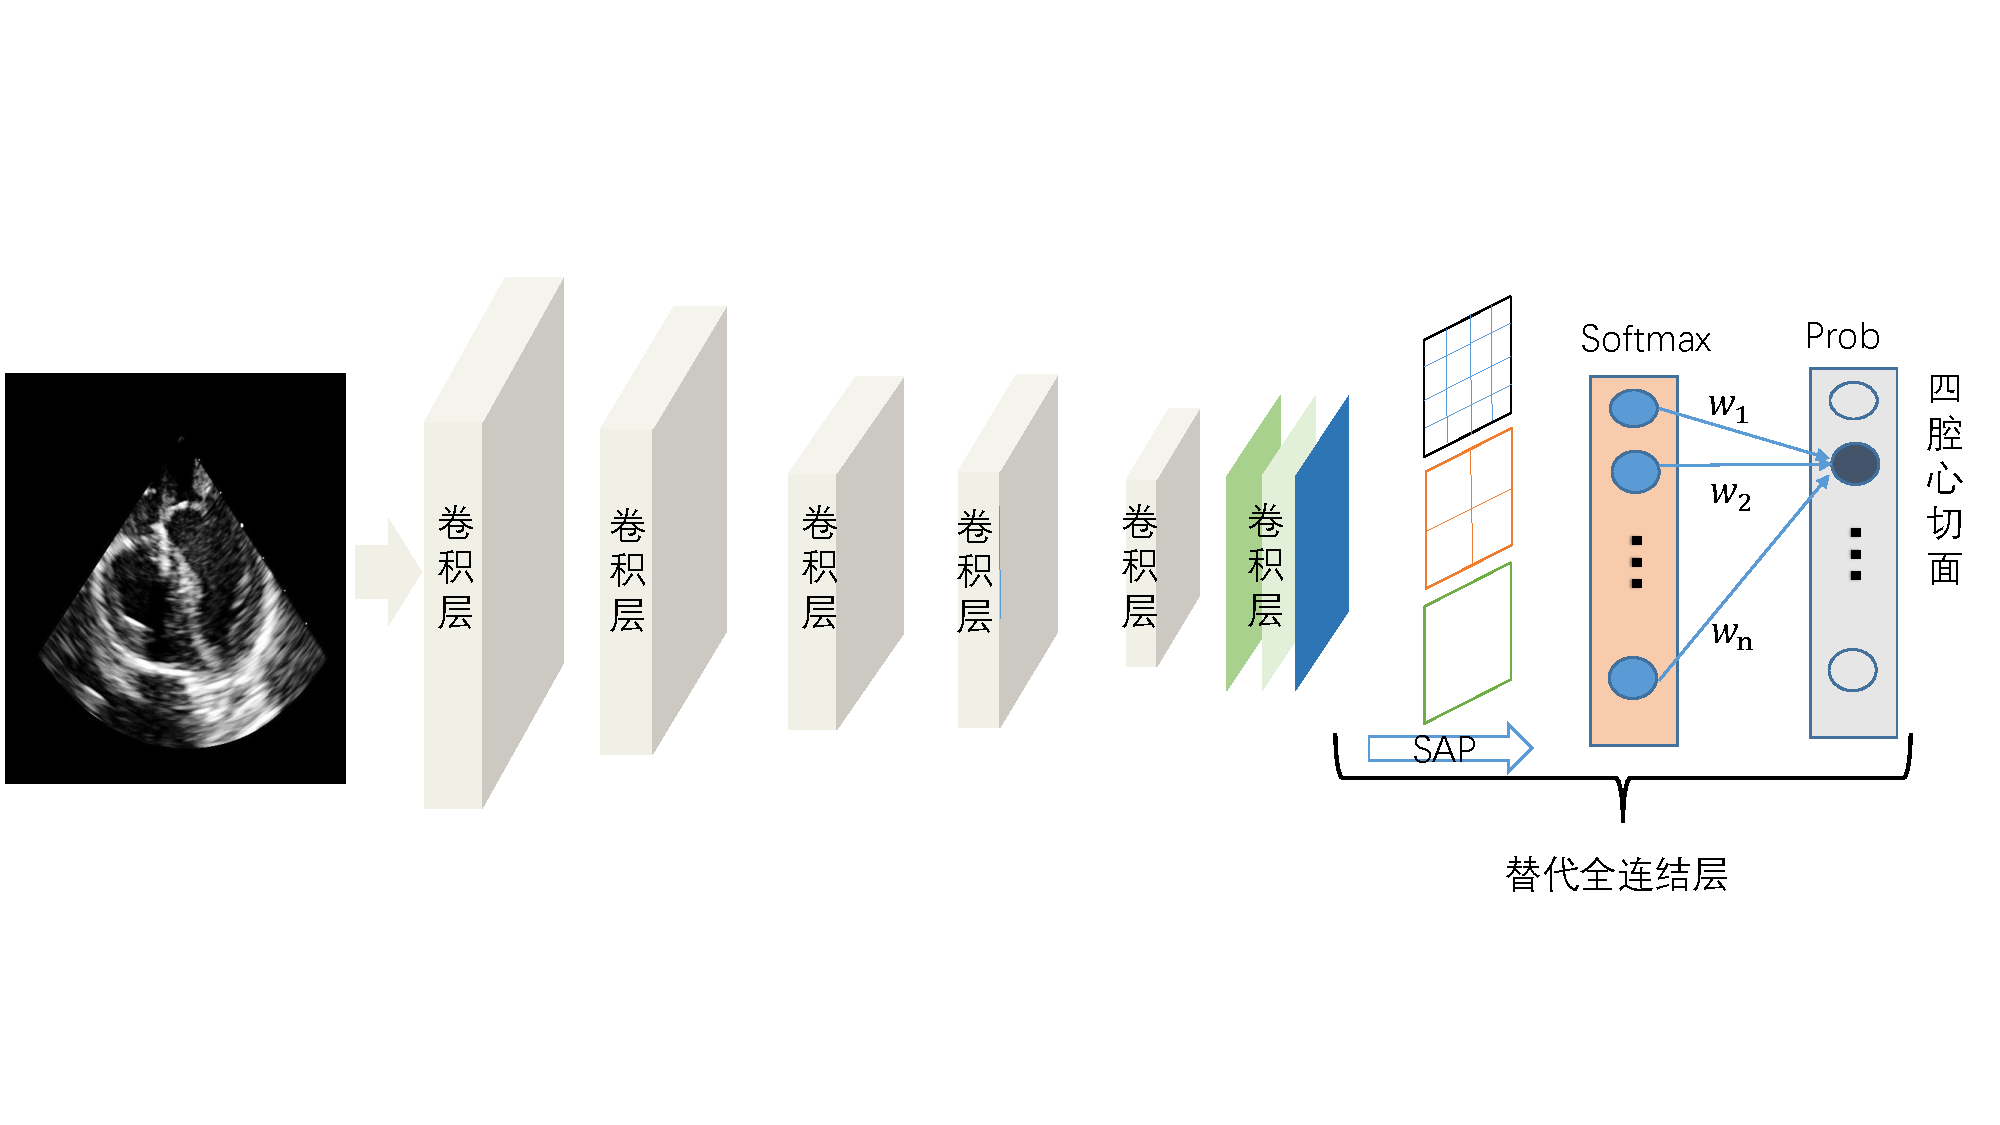
\includegraphics[trim = 30mm 0mm 30mm 0mm, clip, width=0.45\textwidth]{ch03_02}
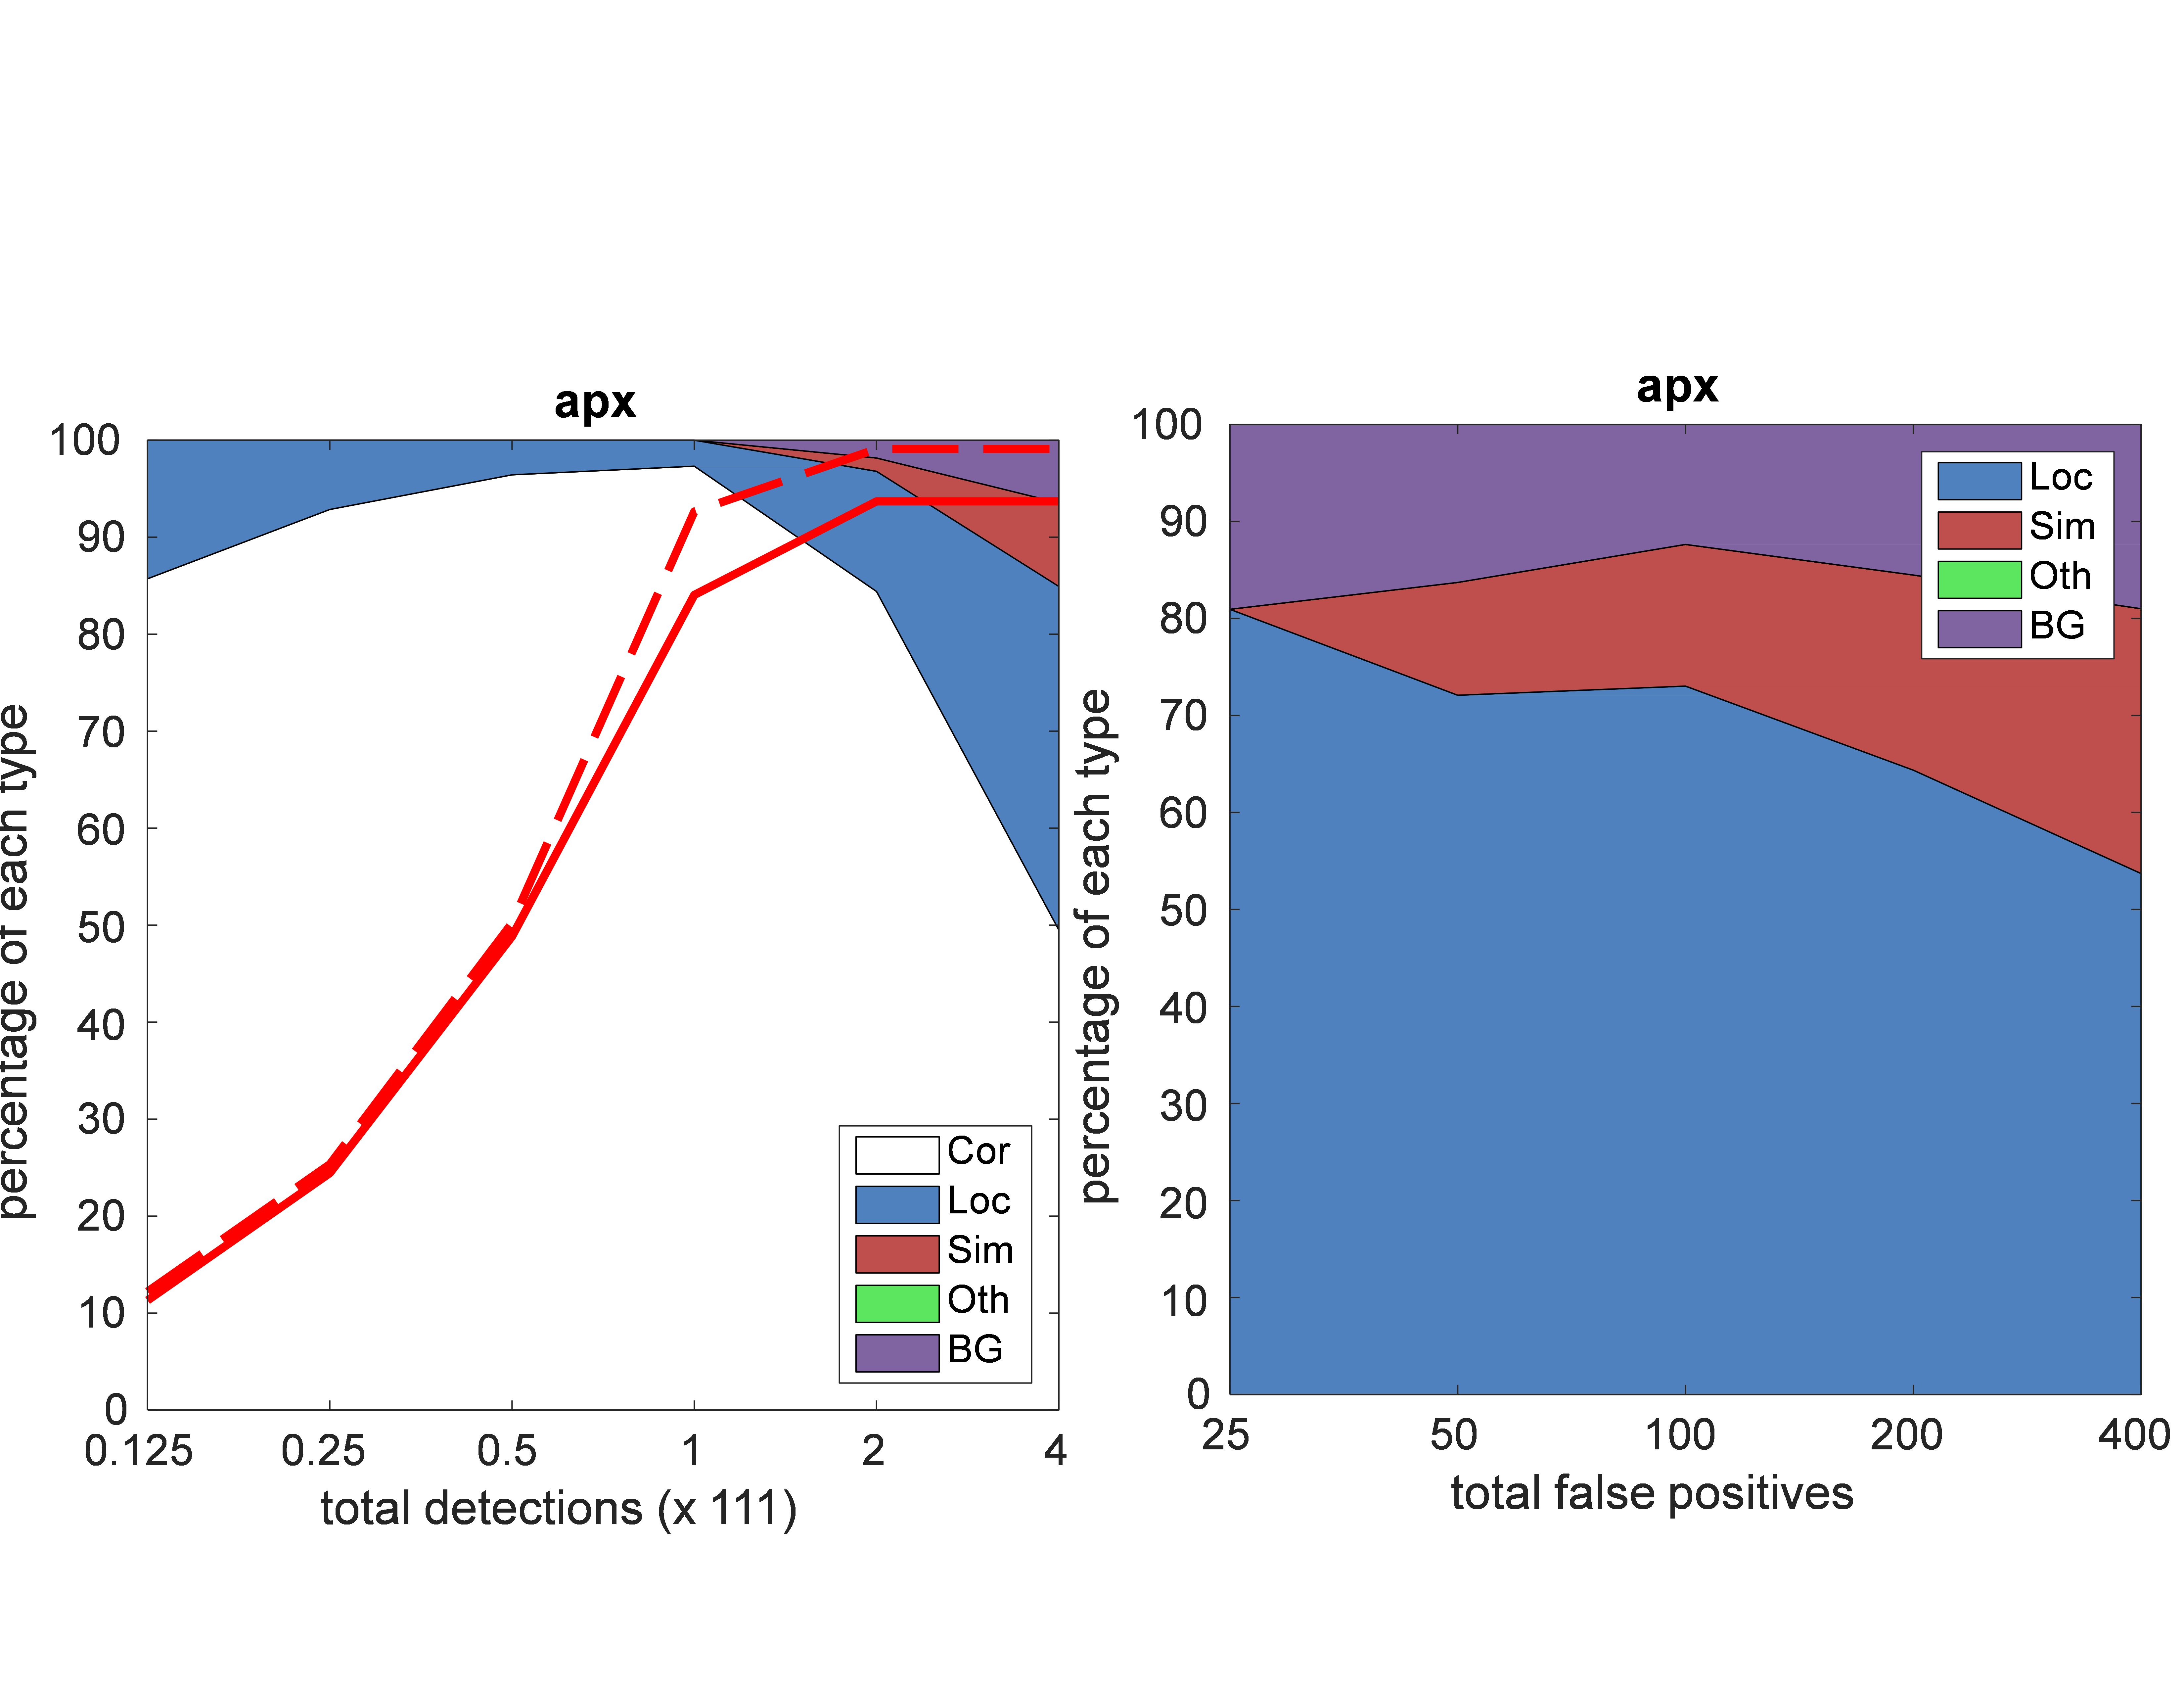
\includegraphics[width=0.85\textwidth]{ch05_03}
\caption{左图显示apx检测精度的累积分布:正确的(Cor)或定位不准确(Loc)的假阳性,与之混淆类似类别(Sim)与其他类别(Oth)或背景(BG)。固体红色线是以“强”标准(大于0.5 交叠比),反映精确度随检测增加而变化。红色虚线使用“弱”标准(大于0.1交叠比)。右图显示排名靠前的假阳性类型的分布。}
\label{fig:ch05_03}
\end{figure} 	                          
 
\begin{figure}[!htbp]
\centering
%trim option's parameter order: left bottom right top
%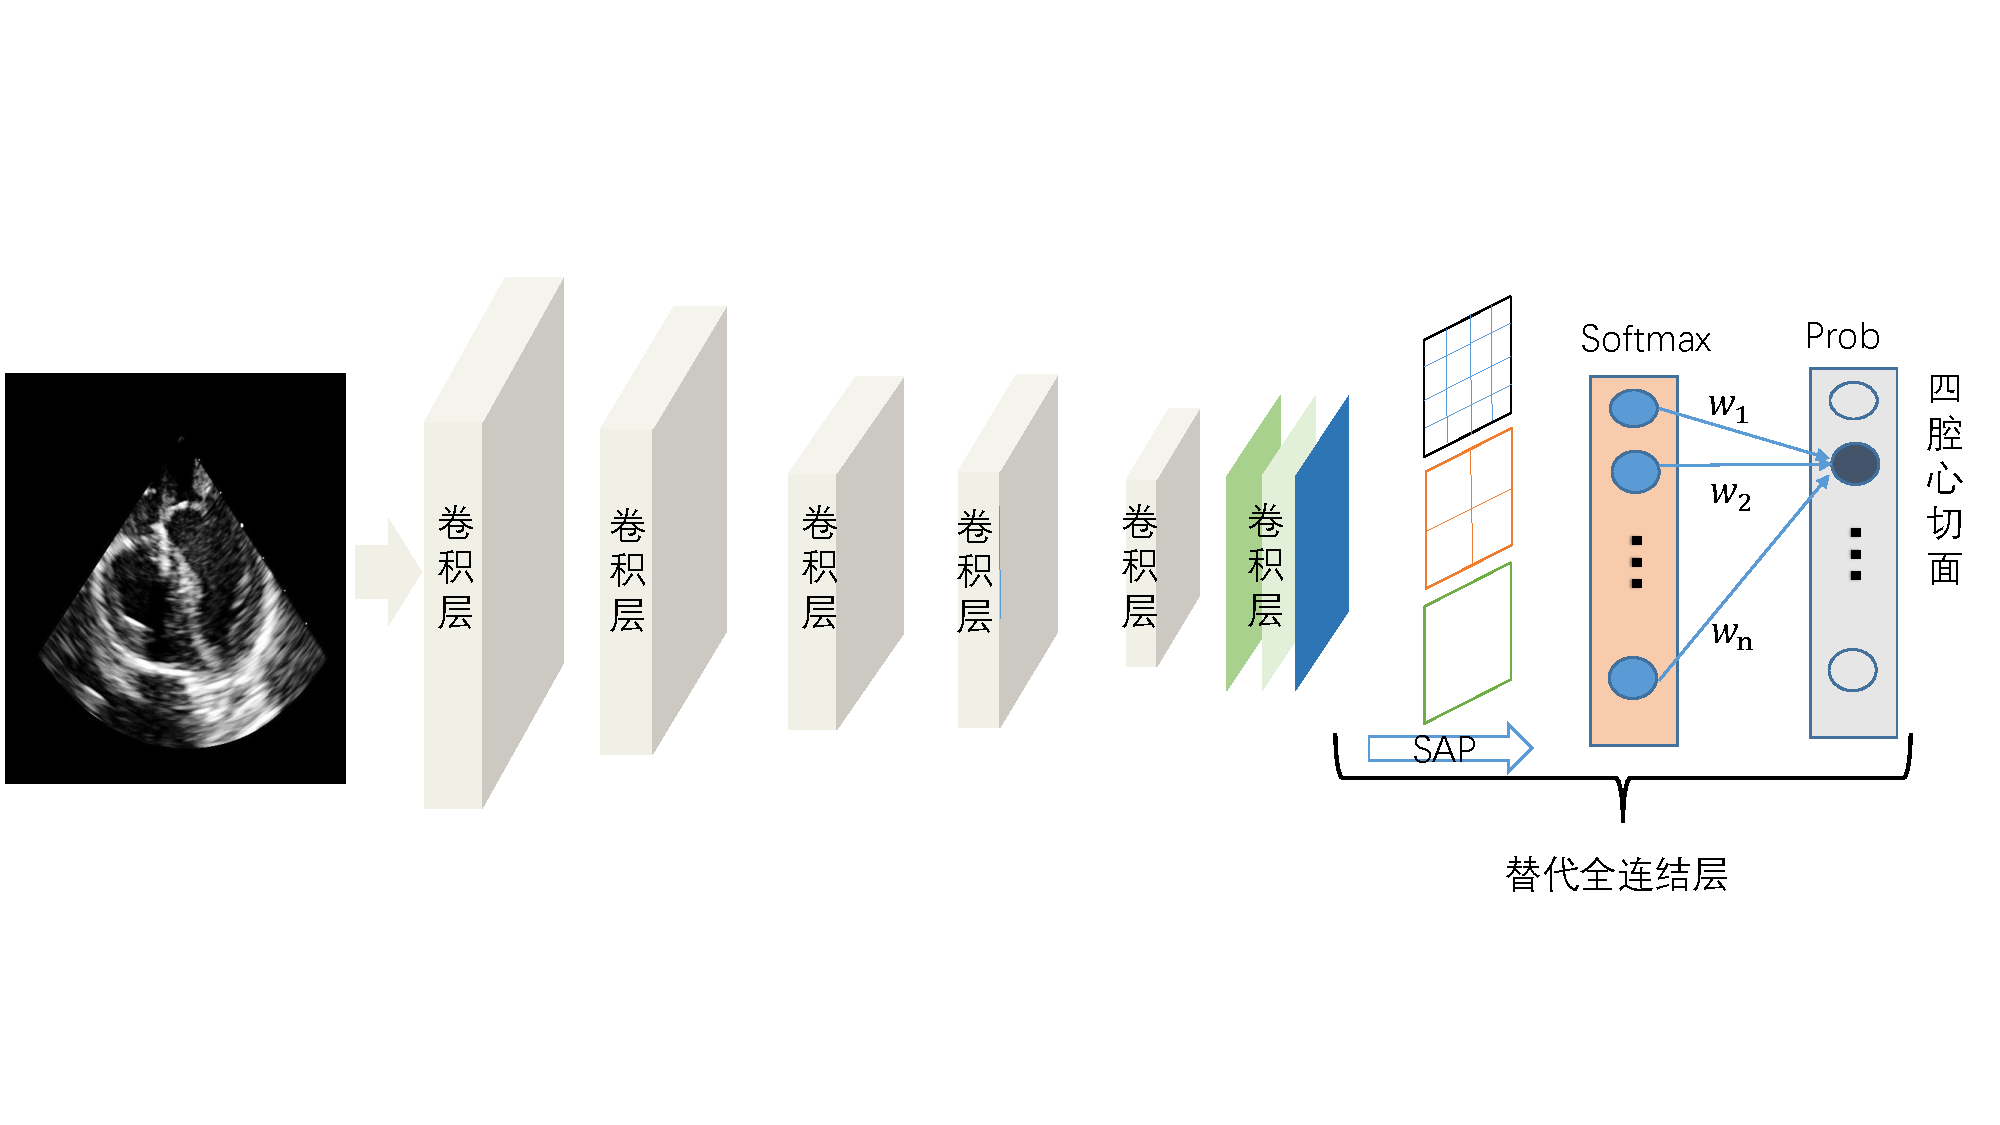
\includegraphics[trim = 30mm 0mm 30mm 0mm, clip, width=0.45\textwidth]{ch03_02}
\includegraphics[width=0.85\textwidth]{ch05_04}
\caption{(a,b) 表示不同MRI图像检测左心室结果,(c,d)两图表示超声心动图的ME4C切面的左心室、二尖瓣环、心内膜垫和心尖位置及旋转角度的检测结果。}
\label{fig:ch05_04}
\end{figure} 	                         
 
\section{小结与讨论}

本文利用深度学习来解决医学图像计算机辅助检测问题,设计并验证了自动检测MRI短轴和超声心动图中LV长轴切面的方法,在通用物体检测Faster RCNN框架的基础上,针对RPN引入空间变换,结合带朝向损失的多任务损失,探索解决图像平面内物体旋转角度检测的问题,并利用困难样例挖掘策略加快迭代训练。在公共MRI数据集和自主收集的超声心动图数据上进行详尽实验验证,在多个评估指标方面提供更好的测试结果,但该方法仍耗费较多的标注数据,探索需要更少标注数据的检测算法是将来的工作目标。